\subsection{Méthode graphique}
Soit l'échantillon aléatoire $X_1$,...,$X_n$ obtenu avec la loi de densité suivante (définie pour $x \geq 0$, avec $k$ et $c > 0$) :
$$ f(x) = \frac{k}{c}\left(\frac{x}{c}\right)^{k-1}\exp\left[-\left(\frac{x}{c}\right)^{k}\right] $$ 
On aimerait trouver un estimateur $\hat{\theta} = (\hat{k},\hat{c})$ pour $\theta = (k,c)$ en utilisant la régression linéaire.\\
Pour cela, notons que
$$ \ln(-\ln(1-F(x))) = k\ln(x)-k\ln(c) $$
Il suffit alors de choisir des points $x$ et d'estimer $F(x)$ grâce aux données empiriques $X_1$,...,$X_n$. La régression linéaire nous donnera des estimateurs $\hat{k}$ et $-\hat{k}\ln(\hat{c})$ dont nous pouvons facilement extraire $\hat{\theta}$. Pour simplifier les choses, on peut réindicer $X_1$,...,$X_n$ en $X_1'$,...,$X_n'$, de telle sorte que $X_1'<X_2'<$...$<X_n'$ (on suppose les $X_i$ obtenus différents). On évalue alors très simplement $F$ en chaque $X_i'$ : 
$$ \hat{F}(X_i') = i/n $$
On peut alors utiliser les $n-1$ premières valeurs de $X'$ pour effectuer la régression linéaire (le soucis avec la dernière c'est que $\hat{F}(X_n') = 1$ et donc $\ln(1-F)$ n'est pas défini). Par symétrie, il semble logique de rejeter aussi la première valeur (bien que la distribution Weibull ne soit pas symétrique). Voir code matlab pour l'implémentation.
\paragraph{}
Pour la suite, nous avons choisi $\theta = (2,2)$ comme paramètres à estimer et $n =1000$ comme taille d'échantillon.
Nous calculons $\hat{\theta}$ avec la régression linéaire, puis l'erreur quadratique totale $ERT$.\\
Voici les résultats obtenus pour un échantillon particulier (voir figure~\ref{fig:droite} pour la droite de régression linéaire) :
$$ \hat{\theta} = (1.9872,2.0368) \text{ et } ERT  = 0.0015 $$

\begin{figure}[!ht]
        \centering
        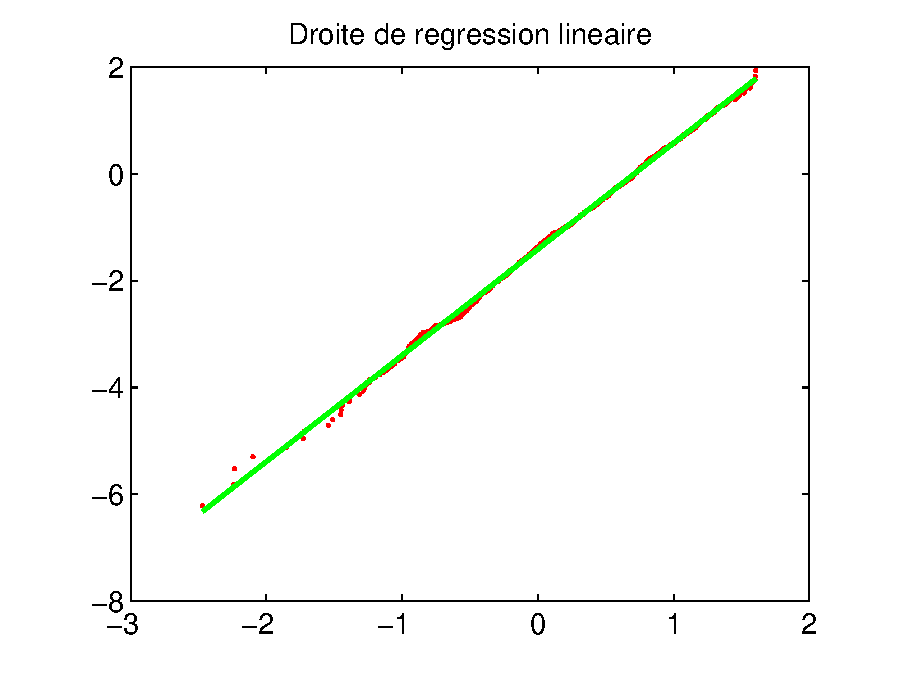
\includegraphics[width=0.4\textwidth]{graphes/droite_mg.eps}
        \caption{Droite de régression}\label{fig:droite}
\end{figure}

Pour étudier le biais et la variance de notre estimateur, nous avons reproduit notre estimation sur 500 échantillons. Voici les résultat pour la moyenne et la variance des séries $\hat{k}$, $\hat{c}$ et $ERT$. Les valeurs obtenues sont reprises dans la table~\ref{table:reg1}.

\begin{table}[!ht]
\centering
\begin{tabular}{|l|l|l|}
\hline
				& Moyenne 	& Variance\\
\hline
$\hat{k}$ 	& $1.9866$ 	& $0.0044$\\
$\hat{c}$ 	& $2.0020$ 	& $0.0012$\\
$ERT$		& $0.0057$	& $4.0814\cdot 10^{-5}$\\
\hline
\end{tabular}
\caption{Table des valeurs obtenues avec la méthode de régression linéaire pour 500 échantillons.}
\label{table:reg1}
\end{table}

Pour chaque série, nous avons produit un box-plot et un histogramme. Les graphes relatifs à $\hat{k}$ se retrouvent à la figure~\ref{fig:kmg}, ceux de $\hat{c}$ à la figure~\ref{fig:cmg} et ceux de $ERT$ à la figure~\ref{fig:ertmg}.

\begin{figure}[!ht]
        \centering
        \begin{subfigure}[b]{0.4\textwidth}
                \includegraphics[width=\textwidth]{graphes/boxplot_kmg.eps}
        \end{subfigure}%
        ~
        \begin{subfigure}[b]{0.4\textwidth}
                \includegraphics[width=\textwidth]{graphes/hist_kmg.eps}
        \end{subfigure}
        \caption{Graphes pour $\hat{k}$}\label{fig:kmg}
\end{figure}

\begin{figure}[!ht]
        \centering
        \begin{subfigure}[b]{0.4\textwidth}
                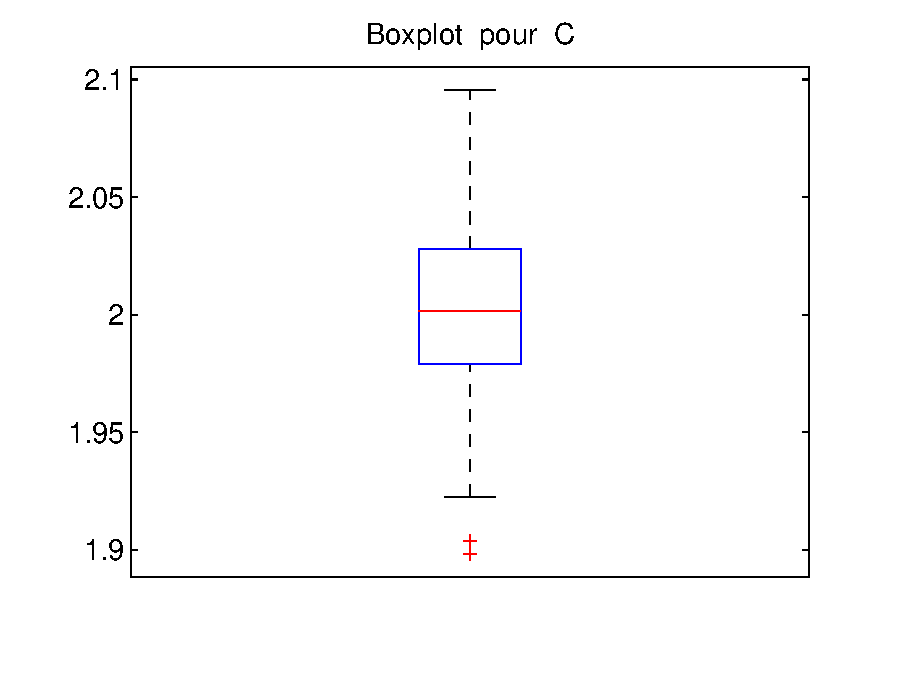
\includegraphics[width=\textwidth]{graphes/boxplot_cmg.eps}
        \end{subfigure}%
        ~
        \begin{subfigure}[b]{0.4\textwidth}
                \includegraphics[width=\textwidth]{graphes/hist_cmg.eps}
        \end{subfigure}
        \caption{Graphes pour $\hat{c}$}\label{fig:cmg}
\end{figure}

\begin{figure}[!ht]
        \centering
        \begin{subfigure}[b]{0.4\textwidth}
                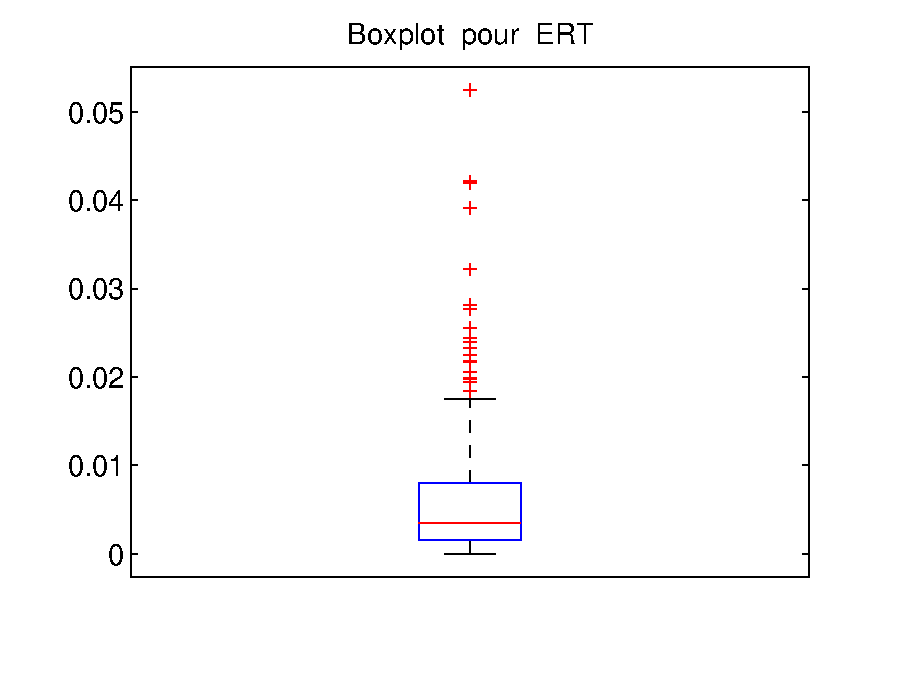
\includegraphics[width=\textwidth]{graphes/boxplot_ertmg.eps}
        \end{subfigure}%
        ~ 
        \begin{subfigure}[b]{0.4\textwidth}
                \includegraphics[width=\textwidth]{graphes/hist_ertmg.eps}
        \end{subfigure}
        \caption{Graphes pour $ERT$}\label{fig:ertmg}
\end{figure}

On ne peut pas dire avec certitude que notre estimateur est biaisé ou non. Si on devait estimer $\beta_0$ et $\beta_1$ tirés d'un modèle de type $Y = \beta_0 + \beta_1x + \epsilon$ avec $\epsilon$ venant d'une certaine distribution de moyenne nulle, alors la théorie prédit que les estimateurs fournis par la régression linéaire pour $\beta_0$ et $\beta_1$ sont non biaisés. Cependant, ici rien ne garantit la condition sur $\epsilon$, on va donc s'en tenir aux observations pour dire si nos estimateurs sont biaisés ou non.\\
Nous observons que notre estimateur pour $k$ est biaisé, tandis que celui pour $c$ ne l'est pas, du moins approximativement. Pour réduire le biais de $\hat{k}$ par rapport à $k$, on peut prendre des échantillons plus grands. On a aussi observé que rejeter plus de valeurs extrêmes réduisait le biais. Voici par exemples les résultat pour $n=10000$ en rejetant la première et dernière valeur (table~\ref{table:reg2}), et les résultats pour $n=1000$ en rejetant les 10 premières et les 10 dernières valeurs (table~\ref{table:reg10}).

\begin{table}[!ht]
\centering
\begin{tabular}{|l|l|l|}
\hline
				& Moyenne 	& Variance\\
\hline
$\hat{k}$ 	& $1.9960$ 	& $4.0303\cdot10^{-4}$\\
$\hat{c}$ 	& $1.9998$ 	& $1.1791\cdot10^{-4}$\\
$ERT$		& $5.3600\cdot10^{-4}$	& $3.5441\cdot 10^{-7}$\\
\hline
\end{tabular}
\caption{Régression linéaire, $n=10000$.}
\label{table:reg2}
\end{table}

\begin{table}[!ht]
\centering
\begin{tabular}{|l|l|l|}
\hline
				& Moyenne 	& Variance\\
\hline
$\hat{k}$ 	& $1.9924$ 	& $0.0035$\\
$\hat{c}$ 	& $1.9966$ 	& $0.0012$\\
$ERT$		& $0.0035$	& $2.2722\cdot 10^{-5}$\\
\hline
\end{tabular}
\caption{Régression linéaire, $n=1000$, valeurs extrêmes rejetées.}
\label{table:reg10}
\end{table}

Le résultat pour $n=10000$ montre que bien que $\hat{k}$ soit biaisé, il est asymptotiquement non biaisé. \\
Pour ce qui est de la distribution asymptotique de nos estimateurs, on peut voir dans les histogrammes (figures ~\ref{fig:kmg} et ~\ref{fig:cmg}) qu'elle est approximativement normale. \`A nouveau, si on avait pu affirmer se retrouver dans le cas d'un modèle de type $Y = \beta_0 + \beta_1x + \epsilon$, avec cette fois-ci $\epsilon$ distribué normalement et de moyenne nulle, alors la théorie prédit que les estimateurs pour $\beta_0$ et $\beta_1$ sont distribués normalement.\\
Enfin, on peut raisonnablement affirmer que nos estimateurs sont consistants, sachant que $\hat{c}$ est non biaisé, $\hat{k}$ est asymptotiquement non biaisé, et pour tous deux la variance tend vers $0$ lorsque $n$ tend vers l'infini.
